\documentclass[10pt]{article}
\usepackage{NotesTeX} %/Path/to/package should be replaced with package location
\usepackage{lipsum}
\usepackage{tensor}
\usepackage{amsmath,amsthm,amssymb}
\usepackage{hyperref}
\usepackage{gensymb}
\usepackage{subcaption}
\usepackage{wrapfig}
\usepackage{float}

\newcommand{\bs}{\textbackslash}


\title{{\Huge General Relativity}\\{\Large{Class 15 -- February 21, 2020}}} %replace with class number
\author{Stacie Moltner}

\emailAdd{staciemoltner@utexas.edu} %replace with your email
\begin{document}
\maketitle
\flushbottom
\newpage
\pagestyle{fancynotes}


\section{Orbits Around Spherically Symmetric Black Holes}\label{sec:orbits}
\begin{itemize}
\item Line element for a spherically symmetric black hole, or Schwarzschild black hole:
\begin{equation}
ds^2 = -\left(1-\dfrac{2M}{r}\right)dt^2 + \dfrac{dr^2}{1-\frac{2M}{r}} + r^2 d\Omega^2,
\end{equation}
where $M$ is the mass of the black hole in units of $G=c=1$.

Note: to convert $M$ back to SI units of mass, replace by conversion factor $\frac{GM}{c^2}$.

\item Placing spherical shells around the black hole and labelling each shell by its radius (Figure \ref{fig:shells}), corresponding to coordinate $r$, observers on a shell will measure proper time
\begin{equation}
d\tau = \left(1-\dfrac{2M}{r}\right)^{\frac{1}{2}} dt,
\end{equation}
and distance between shells
\begin{equation}
ds = \dfrac{dr}{\left(1-\frac{2M}{r}\right)^\frac{1}{2}}.
\end{equation}
Clocks on the shell will run slower than clocks far away, and distances measured on the shell will be larger than measured from far away.

\begin{figure}[h]\label{fig:shells}
\centering
\tikzset{every picture/.style={line width=0.75pt}} %set default line width to 0.75pt        

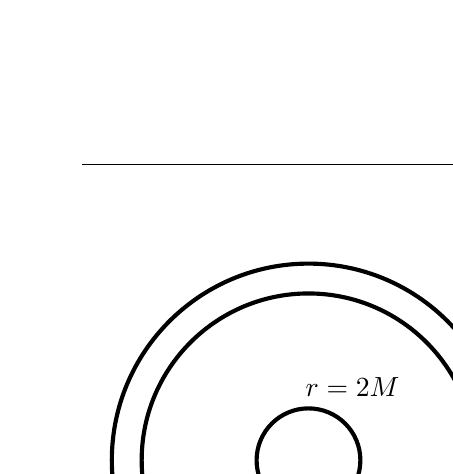
\begin{tikzpicture}[x=0.75pt,y=0.75pt,yscale=-1,xscale=1]
%uncomment if require: \path (0,300); %set diagram left start at 0, and has height of 300

%Shape: Circle [id:dp00569042670082609] 
\draw  [line width=1.5]  (89.75,165.25) .. controls (89.75,151.44) and (100.94,140.25) .. (114.75,140.25) .. controls (128.56,140.25) and (139.75,151.44) .. (139.75,165.25) .. controls (139.75,179.06) and (128.56,190.25) .. (114.75,190.25) .. controls (100.94,190.25) and (89.75,179.06) .. (89.75,165.25) -- cycle ;
%Shape: Circle [id:dp011870213663315088] 
\draw  [line width=1.5]  (20,165.25) .. controls (20,112.92) and (62.42,70.5) .. (114.75,70.5) .. controls (167.08,70.5) and (209.5,112.92) .. (209.5,165.25) .. controls (209.5,217.58) and (167.08,260) .. (114.75,260) .. controls (62.42,260) and (20,217.58) .. (20,165.25) -- cycle ;
%Shape: Circle [id:dp17328455139373267] 
\draw  [line width=1.5]  (34.38,165.25) .. controls (34.38,120.86) and (70.36,84.88) .. (114.75,84.88) .. controls (159.14,84.88) and (195.13,120.86) .. (195.13,165.25) .. controls (195.13,209.64) and (159.14,245.63) .. (114.75,245.63) .. controls (70.36,245.63) and (34.38,209.64) .. (34.38,165.25) -- cycle ;
%Straight Lines [id:da5026773640476042] 
\draw [line width=1.5]    (146.75,238.63) -- (153.21,252.3) ;

% Text Node
\draw (136,130) node   [align=left] {{\fontfamily{helvet}\selectfont $r = 2M$}};
% Text Node
\draw (86,230) node   [align=left] {$r_1$};
% Text Node
\draw (76,262) node   [align=left] {$r_2$};
% Text Node
\draw (158,262) node   [align=left] {$ds$};
\end{tikzpicture}
\caption{Spherical shells at $r=r_1,r_2$ surrounding the black hole horizon at $r=2M$. Distances between shells are measured by $ds$.}
\end{figure}

\item In orbits around black holes, specific energy and specific angular momentum are conserved quantities on trajectories subject only to the forces of curved spacetime (i.e. geodesics):
\begin{align}
\text{Specific energy:}& \qquad \mathcal{E} = \dfrac{E}{m}.
\\
\text{Specific angular momentum:}& \qquad \mathcal{L} = \dfrac{L}{m} = r^2 \dfrac{d\phi}{d\tau}.
\end{align}

\item Recall that the tangent to the curve travelled by a particle is given by $U^\mu = \frac{dx^\mu}{d\tau}$, %satisfying $U^\mu U^\nu g_{\mu\nu} = -1$,
from which we can derive:
\begin{equation}
\mathcal{E}^2 = \left(\dfrac{dr}{d\tau}\right)^2 + V_\text{eff},
\end{equation}
where $\frac{dr}{d\tau}$ is the radial velocity and $V_\text{eff}$ is the effective potential:
\begin{equation}\label{eq:veff_bh_1}
V_\text{eff} = \left(1-\dfrac{2M}{r}\right)\left(1+\dfrac{\mathcal{L}^2}{r^2}\right).
\end{equation}

\item
Comparing this to energy and effective potential in the Newtonian case of a spherically symmetric gravitational potential,
\begin{align}
&E = \dfrac{1}{2}m\dot{r}^2 + V_\text{eff},
\\
&V_\text{eff} = -\dfrac{2Mm}{r} + \dfrac{L^2}{2mr^2}.
\label{eq:veff_newt}
\end{align}

%\end{equation}
%\begin{equation}

Far away, the effective potential is dominated by the first term in Eq.(\ref{eq:veff_newt}), while the second term dominates for small $r$. 

Figure \ref{fig:veff_newt} shows the effective potential as well as possible orbits.
Particles travelling hyperbolic orbits have positive energy, reaching a point of closest approach before turning around.
Elliptical orbits have negative energy, and are bound in orbit.
Circular, stable orbits have zero radial velocity, orbiting at constant radius.

\begin{figure}[h]
\centering
\label{fig:veff}
\begin{subfigure}{0.5\textwidth} \label{fig:veff_newt}
\centering



\tikzset{every picture/.style={line width=0.75pt}} %set default line width to 0.75pt        

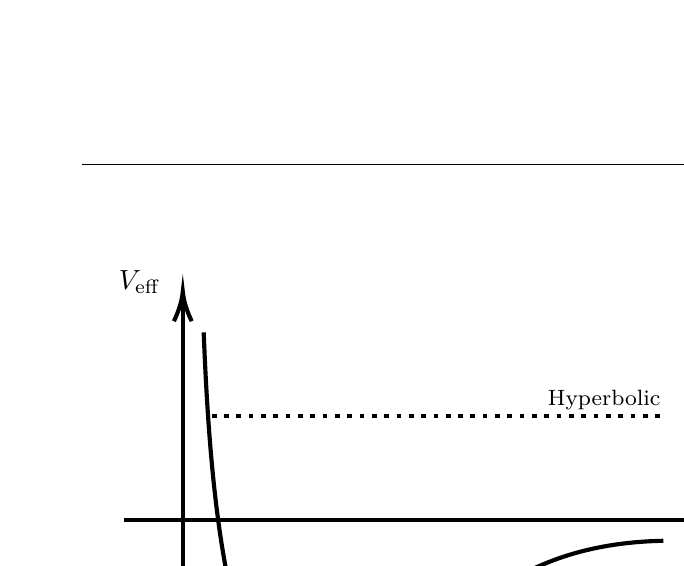
\begin{tikzpicture}[x=0.75pt,y=0.75pt,yscale=-1,xscale=1]
%uncomment if require: \path (0,650); %set diagram left start at 0, and has height of 650

%Straight Lines [id:da9441816186050421] 
\draw [line width=1.5]    (80,250) -- (80,33) ;
\draw [shift={(80,30)}, rotate = 450] [color={rgb, 255:red, 0; green, 0; blue, 0 }  ][line width=1.5]    (14.21,-4.28) .. controls (9.04,-1.82) and (4.3,-0.39) .. (0,0) .. controls (4.3,0.39) and (9.04,1.82) .. (14.21,4.28)   ;
%Straight Lines [id:da9687655051970443] 
\draw [line width=1.5]    (51.5,140) -- (338.5,140) ;
\draw [shift={(341.5,140)}, rotate = 180] [color={rgb, 255:red, 0; green, 0; blue, 0 }  ][line width=1.5]    (14.21,-4.28) .. controls (9.04,-1.82) and (4.3,-0.39) .. (0,0) .. controls (4.3,0.39) and (9.04,1.82) .. (14.21,4.28)   ;
%Curve Lines [id:da8257399427279626] 
\draw [line width=1.5]    (90.07,49.62) .. controls (93.95,150.14) and (105.95,240.14) .. (149.95,240.14) .. controls (193.95,240.14) and (200.95,152.14) .. (311.5,150) ;
%Straight Lines [id:da4141774024729541] 
\draw [line width=1.5]  [dash pattern={on 1.69pt off 2.76pt}]  (94,90) -- (310.17,90) ;
%Straight Lines [id:da5016916420858185] 
\draw [line width=1.5]  [dash pattern={on 5.63pt off 4.5pt}]  (111,202.46) -- (200.93,202.46) ;
%Shape: Circle [id:dp6498127078174468] 
\draw  [fill={rgb, 255:red, 0; green, 0; blue, 0 }  ,fill opacity=1 ] (153.51,240.14) .. controls (153.51,238.18) and (151.92,236.58) .. (149.95,236.58) .. controls (147.99,236.58) and (146.39,238.18) .. (146.39,240.14) .. controls (146.39,242.11) and (147.99,243.7) .. (149.95,243.7) .. controls (151.92,243.7) and (153.51,242.11) .. (153.51,240.14) -- cycle ;
%Curve Lines [id:da23902979172722738] 
\draw    (219.39,231.77) .. controls (211.39,246.77) and (184.39,260.77) .. (155,246.77) ;

% Text Node
\draw (59,25.46) node   [align=left] {$\displaystyle V_\text{eff}$};
% Text Node
\draw (340,126.46) node   [align=left] {$\displaystyle r$};
% Text Node
\draw (283,82) node  [font=\fontsize{0.8em}{0.96em}\selectfont] [align=left] {Hyperbolic};
% Text Node
\draw (179,194) node  [font=\fontsize{0.8em}{0.96em}\selectfont] [align=left] {Elliptical};
% Text Node
\draw (259,223) node  [font=\fontsize{0.8em}{0.96em}\selectfont] [align=left] {Circular (stable)};


\end{tikzpicture}
\subcaption{Newtonian effective potential with possible orbits.}
\end{subfigure}

\begin{subfigure}{0.5\textwidth} \label{fig:veff_gr}
\centering

\tikzset{every picture/.style={line width=0.75pt}} %set default line width to 0.75pt        

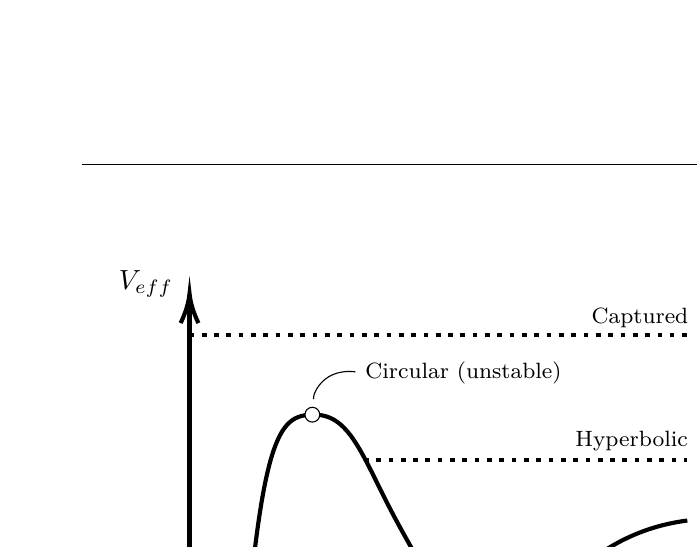
\begin{tikzpicture}[x=0.75pt,y=0.75pt,yscale=-1,xscale=1]
%uncomment if require: \path (0,650); %set diagram left start at 0, and has height of 650

%Straight Lines [id:da40833697820157033] 
\draw [line width=1.5]    (80,500) -- (80,283) ;
\draw [shift={(80,280)}, rotate = 450] [color={rgb, 255:red, 0; green, 0; blue, 0 }  ][line width=1.5]    (14.21,-4.28) .. controls (9.04,-1.82) and (4.3,-0.39) .. (0,0) .. controls (4.3,0.39) and (9.04,1.82) .. (14.21,4.28)   ;
%Straight Lines [id:da5886300795452046] 
\draw [line width=1.5]    (51.5,461) -- (338.5,461) ;
\draw [shift={(341.5,461)}, rotate = 180] [color={rgb, 255:red, 0; green, 0; blue, 0 }  ][line width=1.5]    (14.21,-4.28) .. controls (9.04,-1.82) and (4.3,-0.39) .. (0,0) .. controls (4.3,0.39) and (9.04,1.82) .. (14.21,4.28)   ;
%Curve Lines [id:da7119234455375559] 
\draw [line width=1.5]    (103.89,488.04) .. controls (113.83,347.33) and (122.17,338.33) .. (140.17,338.33) .. controls (158.17,338.33) and (163.83,360.33) .. (180.17,390.33) .. controls (196.5,420.33) and (208.83,440.33) .. (229.83,440.33) .. controls (250.83,440.33) and (265.83,396.33) .. (319.83,389.33) ;
%Straight Lines [id:da8860122903021546] 
\draw [line width=1.5]  [dash pattern={on 1.69pt off 2.76pt}]  (164,360) -- (319.83,360) ;
%Straight Lines [id:da35086257271406274] 
\draw [line width=1.5]  [dash pattern={on 5.63pt off 4.5pt}]  (198,420.46) -- (258.83,420.46) ;
%Shape: Circle [id:dp4670184596858362] 
\draw  [fill={rgb, 255:red, 0; green, 0; blue, 0 }  ,fill opacity=1 ] (233.39,440.33) .. controls (233.39,438.37) and (231.8,436.77) .. (229.83,436.77) .. controls (227.87,436.77) and (226.27,438.37) .. (226.27,440.33) .. controls (226.27,442.3) and (227.87,443.89) .. (229.83,443.89) .. controls (231.8,443.89) and (233.39,442.3) .. (233.39,440.33) -- cycle ;
%Shape: Circle [id:dp8655485684914681] 
\draw  [fill={rgb, 255:red, 255; green, 255; blue, 255 }  ,fill opacity=1 ] (142.73,338.33) .. controls (142.73,336.37) and (141.13,334.77) .. (139.17,334.77) .. controls (137.2,334.77) and (135.61,336.37) .. (135.61,338.33) .. controls (135.61,340.3) and (137.2,341.89) .. (139.17,341.89) .. controls (141.13,341.89) and (142.73,340.3) .. (142.73,338.33) -- cycle ;
%Curve Lines [id:da825883119903197] 
\draw    (275.39,437.77) .. controls (264.39,453.77) and (248.39,454.77) .. (235,446.77) ;
%Curve Lines [id:da894643506405834] 
\draw    (159.92,317.68) .. controls (141.92,315.68) and (138.5,332) .. (140,330.77) ;
%Straight Lines [id:da742508397381557] 
\draw [line width=1.5]  [dash pattern={on 1.69pt off 2.76pt}]  (80,300) -- (320.92,300) ;

% Text Node
\draw (59,275.46) node   [align=left] {$\displaystyle V_{eff}$};
% Text Node
\draw (340,447.46) node   [align=left] {$\displaystyle r$};
% Text Node
\draw (138,450) node   [align=left] {$\displaystyle r=2M$};
% Text Node
\draw (293,351) node  [font=\fontsize{0.8em}{0.96em}\selectfont] [align=left] {Hyperbolic};
% Text Node
\draw (238,412) node  [font=\fontsize{0.8em}{0.96em}\selectfont] [align=left] {Elliptical};
% Text Node
\draw (305,429) node  [font=\fontsize{0.8em}{0.96em}\selectfont] [align=left] {Circular (stable)};
% Text Node
\draw (212,318) node  [font=\fontsize{0.8em}{0.96em}\selectfont] [align=left] {Circular (unstable)};
% Text Node
\draw (297,292) node  [font=\fontsize{0.8em}{0.96em}\selectfont] [align=left] {Captured};;
\end{tikzpicture}
\subcaption{\textbf{Schwarzschild?} effective potential with possible orbits. At $r=2M$, $V_\text{eff}=0$.}
\end{subfigure}
\caption{Effective potentials for the Newtonian and Schwarzschild cases.}
\end{figure}

\item
Expanding the effective potential of the black hole (Eq. (\ref{eq:veff_bh_1})):
\begin{equation}
V_{\text{eff}}= 1 - \dfrac{2M}{r} + \dfrac{\mathcal{L}^2}{r^2} - \dfrac{2M\mathcal{L}^2}{r^3}.
\end{equation}
The first term on the right hand side accounts for the minimum energy of a particle, its rest mass ($E=m \Rightarrow \frac{E}{m}=1$).
Of the remaining terms, the second term on the right dominates at large $r$, while the fourth term dominates at small $r$, close to the black hole.

Figure \ref{fig:veff_gr} shows the effective potential of the Schwarzschild black hole with possible orbits. In addition to hyperbolic, elliptical, and stable circular orbits as in the Newtonian case, there exist unstable circular orbits and captured orbits. Given a little bit of energy, particles in unstable circular orbits will travel out to infinity, or fall into the black hole. Particles in captured orbits fall into the black hole.

\end{itemize}
    	
    		
\section{Beyond the Horizon}\label{sec:beyondhorizon}
\begin{itemize}
\item In Schwarzschild coordinates we've been unable to go beyond the horizon because the metric becomes singular at $r=2M$. Choosing a new set of coordinates, we can transform the metric to one which has no singularity at $r=2M$.

\item We can find a new coordinate system by considering the paths of light rays traveling into the black hole. Coordinates travelling along light rays are called null coordinates.
%From the perspective of the $(t,r)$ coordinates, light rays will appear to pile up at the horizon, though the light itself travels into the horizon.

\subsection{Null Coordinates in Flat Spacetime}
For a light ray travelling radially in flat space,
\begin{equation}\label{eq:nullray}
\dfrac{dt}{dr}=\pm 1,
\end{equation}
which has solution $t \pm r = \text{constant}$.
On a spacetime diagram, these represent $45\degree$ lines:
\begin{align}
&u = t-r,
\\
&v = t+r,
\end{align}
shown in Figure \ref{fig:const_u_v}.
\begin{figure}[h]\label{fig:const_u_v}
\centering
\tikzset{every picture/.style={line width=0.75pt}} %set default line width to 0.75pt        

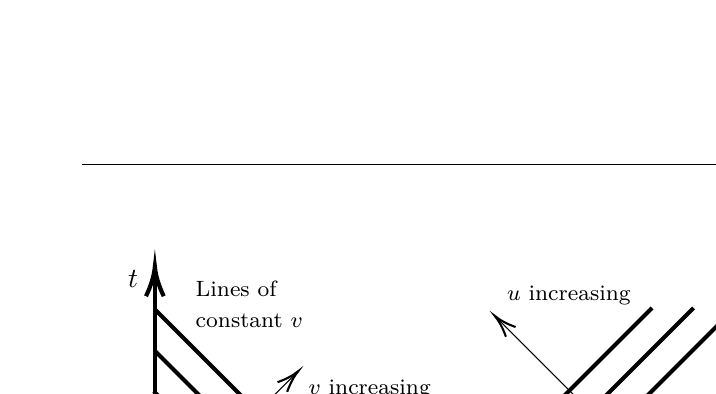
\begin{tikzpicture}[x=0.75pt,y=0.75pt,yscale=-1,xscale=1]
%uncomment if require: \path (0,300); %set diagram left start at 0, and has height of 300

%Straight Lines [id:da5722185969021005] 
\draw [line width=1.5]    (120.5,259.61) -- (120.5,102.96) ;
\draw [shift={(120.5,99.96)}, rotate = 450] [color={rgb, 255:red, 0; green, 0; blue, 0 }  ][line width=1.5]    (14.21,-4.28) .. controls (9.04,-1.82) and (4.3,-0.39) .. (0,0) .. controls (4.3,0.39) and (9.04,1.82) .. (14.21,4.28)   ;
%Straight Lines [id:da5661439418090585] 
\draw [line width=1.5]    (99.76,240.03) -- (407.11,240.03) ;
\draw [shift={(410.11,240.03)}, rotate = 180] [color={rgb, 255:red, 0; green, 0; blue, 0 }  ][line width=1.5]    (14.21,-4.28) .. controls (9.04,-1.82) and (4.3,-0.39) .. (0,0) .. controls (4.3,0.39) and (9.04,1.82) .. (14.21,4.28)   ;
%Straight Lines [id:da7647157962680482] 
\draw [line width=1.5]    (120,160) -- (200.42,240.42) ;
\draw [shift={(160.21,200.21)}, rotate = 45] [fill={rgb, 255:red, 0; green, 0; blue, 0 }  ][line width=0.08]  [draw opacity=0] (11.61,-5.58) -- (0,0) -- (11.61,5.58) -- cycle    ;
%Straight Lines [id:da7829854491463476] 
\draw [line width=1.5]    (120.43,140.43) -- (219.42,239.42) ;
\draw [shift={(169.93,189.93)}, rotate = 45] [fill={rgb, 255:red, 0; green, 0; blue, 0 }  ][line width=0.08]  [draw opacity=0] (11.61,-5.58) -- (0,0) -- (11.61,5.58) -- cycle    ;
%Straight Lines [id:da29078029443885445] 
\draw [line width=1.5]    (239.42,240.42) -- (360.04,119.8) ;
\draw [shift={(299.73,180.11)}, rotate = 495] [fill={rgb, 255:red, 0; green, 0; blue, 0 }  ][line width=0.08]  [draw opacity=0] (11.61,-5.58) -- (0,0) -- (11.61,5.58) -- cycle    ;
%Straight Lines [id:da644885109375044] 
\draw [line width=1.5]    (120.43,120.43) -- (240.42,240.42) ;
\draw [shift={(180.43,180.43)}, rotate = 45] [fill={rgb, 255:red, 0; green, 0; blue, 0 }  ][line width=0.08]  [draw opacity=0] (11.61,-5.58) -- (0,0) -- (11.61,5.58) -- cycle    ;
%Straight Lines [id:da755268462922307] 
\draw [line width=1.5]    (259.42,240.42) -- (380.04,119.8) ;
\draw [shift={(319.73,180.11)}, rotate = 495] [fill={rgb, 255:red, 0; green, 0; blue, 0 }  ][line width=0.08]  [draw opacity=0] (11.61,-5.58) -- (0,0) -- (11.61,5.58) -- cycle    ;
%Straight Lines [id:da4481297569386541] 
\draw [line width=1.5]    (279.42,240.42) -- (400.04,119.8) ;
\draw [shift={(339.73,180.11)}, rotate = 495] [fill={rgb, 255:red, 0; green, 0; blue, 0 }  ][line width=0.08]  [draw opacity=0] (11.61,-5.58) -- (0,0) -- (11.61,5.58) -- cycle    ;
%Straight Lines [id:da558337311834136] 
\draw    (159.93,179.93) -- (188.24,151.62) ;
\draw [shift={(189.65,150.2)}, rotate = 495] [color={rgb, 255:red, 0; green, 0; blue, 0 }  ][line width=0.75]    (10.93,-3.29) .. controls (6.95,-1.4) and (3.31,-0.3) .. (0,0) .. controls (3.31,0.3) and (6.95,1.4) .. (10.93,3.29)   ;
%Straight Lines [id:da15448502747119763] 
\draw    (329.73,169.11) -- (285.65,125.02) ;
\draw [shift={(284.23,123.61)}, rotate = 405] [color={rgb, 255:red, 0; green, 0; blue, 0 }  ][line width=0.75]    (10.93,-3.29) .. controls (6.95,-1.4) and (3.31,-0.3) .. (0,0) .. controls (3.31,0.3) and (6.95,1.4) .. (10.93,3.29)   ;

% Text Node
\draw (166,118) node  [font=\fontsize{0.8em}{0.96em}\selectfont] [align=left] {Lines of\\constant $\displaystyle v$};
% Text Node
\draw (380,189.06) node  [font=\fontsize{0.8em}{0.96em}\selectfont] [align=left] {Lines of\\constant $\displaystyle u$};
% Text Node
\draw (110,106) node   [align=left] {$\displaystyle t$};
% Text Node
\draw (409,227) node   [align=left] {$\displaystyle r$};
% Text Node
\draw (224,159) node  [font=\fontsize{0.8em}{0.96em}\selectfont] [align=left] {$\displaystyle v$ increasing};
% Text Node
\draw (320,114) node  [font=\fontsize{0.8em}{0.96em}\selectfont] [align=left] {$\displaystyle u$ increasing};


\end{tikzpicture}
\caption{}
\end{figure}

\subsection{Null Coordinates in Black Hole Spacetime}
For black holes, we previously found 
\begin{equation}
\dfrac{dt}{dr} = \pm \left(1-\dfrac{2M}{r}\right)^{-1}.
\end{equation}
Defining $f \equiv \left(1-\dfrac{2M}{r}\right)$, and using the chain rule with new coordinate $r_*$, we can write
\begin{equation}
\dfrac{dt}{dr} = \dfrac{dt}{dr_*} \dfrac{dr_*}{dr}=\pm f^{-1}.
\end{equation}
If we insist that
\begin{equation}\label{eq:drstar}
\frac{dr_*}{dr}= f^{-1},
\end{equation}
we have  $\frac{dt}{dr_*} = \pm 1$, with $t\pm r_*=\text{constant}$, analogous to Eq. (\ref{eq:nullray}). Redefining $u,v$ using new coordinate $r_*$:
\begin{align}
&u = t-r_*,
\\ &v = t+r_*.
\end{align}
Along outgoing (incoming) null rays, $u$ ($v$) is constant while $v$ ($u$) changes.


Solving Eq. (\ref{eq:drstar}):
\begin{align}
\dfrac{dr^*}{dr} &= f^{-1} 
\\ &= \dfrac{1}{1-\frac{2M}{r}} 
\\ &= \dfrac{r}{r-2M}
\end{align}

\begin{equation}
r_* = r + 2M \log\left(\dfrac{r}{2M}-1\right)
\end{equation}
$r_*$ is called the \textbf{tortoise coordinate}.

Note that as $r \rightarrow 2M$, $\left(\dfrac{r}{2M}-1\right)\rightarrow 0$, so $r_*\rightarrow -\infty$.
%\begin{align}
%\log\left(\frac{r}{2M}-1\right)\rightarrow -\infty.
%\end{align}

Transforming coordinates to a new coordinate system,
\begin{equation}
x^{\mu '} = (v,r,\theta,\phi),
\end{equation}
counting time by light rays sent into the black hole.

We can transform our coordinate system,
\begin{align}
v&=t+r_* & \Rightarrow & &t=v-r_*
\\r&=r &  &  &r=r,
\end{align}
so the differential $dt$ becomes
\begin{align}
dt&=dv-dr_*
\\ &=dv - \dfrac{dr_*}{dr}dr
\\ &=dv-\dfrac{1}{f}dr.
\end{align}

Transforming the metric,
\begin{align}
ds^2 &= -f\left(dv-\dfrac{dr}{f}\right)^2+\dfrac{dr^2}{f}+r^2 d\Omega
\\ &=-f dv^2 + 2dv dr + r^2 d\Omega^2
\end{align}

Light rays travel along paths $ds^2=0$:
\begin{align}
0 &=f\dfrac{dv^2}{dr^2}+2\dfrac{dv dr}{dr^2}
\\ &=\dfrac{dv}{dr}\left(-f\dfrac{dv}{dr}+2\right),
\end{align}
which has solutions
\begin{align}
\dfrac{dv}{dr} &=
\begin{cases}
0
\\ \frac{2}{f}=2\left(1-\frac{2M}{r}\right)^{-1}.
\end{cases}
\end{align}
In these coordinates, light cones are tilted as shown in Figure \ref{fig:uvlightcones}.
For $r>2M$, there exist trajectories that can travel to large $r$, escaping the black hole. At $r=2M$, one light ray travels along $r=2M$, while all other light rays travel into the black hole. For $r<2M$, both ingoing and outgoing light rays point into the black hole.

\begin{figure}[h]\label{fig:uvlightcones}
\centering


% Gradient Info
  
\tikzset {_235qclqd4/.code = {\pgfsetadditionalshadetransform{ \pgftransformshift{\pgfpoint{0 bp } { 0 bp }  }  \pgftransformscale{1 }  }}}
\pgfdeclareradialshading{_hx5zxwhfw}{\pgfpoint{0bp}{0bp}}{rgb(0bp)=(1,1,1);
rgb(0bp)=(1,1,1);
rgb(25bp)=(0.82,0.01,0.11);
rgb(400bp)=(0.82,0.01,0.11)}
\tikzset{_wkt9rkgpd/.code = {\pgfsetadditionalshadetransform{\pgftransformshift{\pgfpoint{0 bp } { 0 bp }  }  \pgftransformscale{1 } }}}
\pgfdeclareradialshading{_070bpmikj} { \pgfpoint{0bp} {0bp}} {color(0bp)=(transparent!0);
color(0bp)=(transparent!0);
color(25bp)=(transparent!50);
color(400bp)=(transparent!50)} 
\pgfdeclarefading{_fm43y9f1f}{\tikz \fill[shading=_070bpmikj,_wkt9rkgpd] (0,0) rectangle (50bp,50bp); } 

% Gradient Info
  
\tikzset {_wsfv71rf5/.code = {\pgfsetadditionalshadetransform{ \pgftransformshift{\pgfpoint{0 bp } { 0 bp }  }  \pgftransformscale{1 }  }}}
\pgfdeclareradialshading{_5zqxlp1by}{\pgfpoint{0bp}{0bp}}{rgb(0bp)=(1,1,1);
rgb(0bp)=(1,1,1);
rgb(25bp)=(0.82,0.01,0.11);
rgb(400bp)=(0.82,0.01,0.11)}
\tikzset{_c80r5o3mi/.code = {\pgfsetadditionalshadetransform{\pgftransformshift{\pgfpoint{0 bp } { 0 bp }  }  \pgftransformscale{1 } }}}
\pgfdeclareradialshading{_tc9re09ln} { \pgfpoint{0bp} {0bp}} {color(0bp)=(transparent!0);
color(0bp)=(transparent!0);
color(25bp)=(transparent!50);
color(400bp)=(transparent!50)} 
\pgfdeclarefading{_3wnbsmasd}{\tikz \fill[shading=_tc9re09ln,_c80r5o3mi] (0,0) rectangle (50bp,50bp); } 

% Gradient Info
  
\tikzset {_59nr4uahj/.code = {\pgfsetadditionalshadetransform{ \pgftransformshift{\pgfpoint{0 bp } { 0 bp }  }  \pgftransformscale{1 }  }}}
\pgfdeclareradialshading{_r0aisth5k}{\pgfpoint{0bp}{0bp}}{rgb(0bp)=(1,1,1);
rgb(0bp)=(1,1,1);
rgb(25bp)=(0.82,0.01,0.11);
rgb(400bp)=(0.82,0.01,0.11)}
\tikzset{_mphwf1n87/.code = {\pgfsetadditionalshadetransform{\pgftransformshift{\pgfpoint{0 bp } { 0 bp }  }  \pgftransformscale{1 } }}}
\pgfdeclareradialshading{_ytzkk47v7} { \pgfpoint{0bp} {0bp}} {color(0bp)=(transparent!0);
color(0bp)=(transparent!0);
color(25bp)=(transparent!50);
color(400bp)=(transparent!50)} 
\pgfdeclarefading{_co436xk8n}{\tikz \fill[shading=_ytzkk47v7,_mphwf1n87] (0,0) rectangle (50bp,50bp); } 

% Gradient Info
  
\tikzset {_6gwz3k0ks/.code = {\pgfsetadditionalshadetransform{ \pgftransformshift{\pgfpoint{0 bp } { 0 bp }  }  \pgftransformscale{1 }  }}}
\pgfdeclareradialshading{_okyvnvv9z}{\pgfpoint{0bp}{0bp}}{rgb(0bp)=(1,1,1);
rgb(0bp)=(1,1,1);
rgb(25bp)=(0.82,0.01,0.11);
rgb(400bp)=(0.82,0.01,0.11)}
\tikzset{_gr2yrava6/.code = {\pgfsetadditionalshadetransform{\pgftransformshift{\pgfpoint{0 bp } { 0 bp }  }  \pgftransformscale{1 } }}}
\pgfdeclareradialshading{_w0nli0t3t} { \pgfpoint{0bp} {0bp}} {color(0bp)=(transparent!0);
color(0bp)=(transparent!0);
color(25bp)=(transparent!50);
color(400bp)=(transparent!50)} 
\pgfdeclarefading{_d34i20qb2}{\tikz \fill[shading=_w0nli0t3t,_gr2yrava6] (0,0) rectangle (50bp,50bp); } 

% Gradient Info
  
\tikzset {_0bgngox8j/.code = {\pgfsetadditionalshadetransform{ \pgftransformshift{\pgfpoint{0 bp } { 0 bp }  }  \pgftransformscale{1 }  }}}
\pgfdeclareradialshading{_qtksm99xm}{\pgfpoint{0bp}{0bp}}{rgb(0bp)=(1,1,1);
rgb(0bp)=(1,1,1);
rgb(25bp)=(0.82,0.01,0.11);
rgb(400bp)=(0.82,0.01,0.11)}
\tikzset{_51ds2jx88/.code = {\pgfsetadditionalshadetransform{\pgftransformshift{\pgfpoint{0 bp } { 0 bp }  }  \pgftransformscale{1 } }}}
\pgfdeclareradialshading{_2hcgw078d} { \pgfpoint{0bp} {0bp}} {color(0bp)=(transparent!0);
color(0bp)=(transparent!0);
color(25bp)=(transparent!50);
color(400bp)=(transparent!50)} 
\pgfdeclarefading{_anp9pkkbt}{\tikz \fill[shading=_2hcgw078d,_51ds2jx88] (0,0) rectangle (50bp,50bp); } 

% Gradient Info
  
\tikzset {_f14j6p1ka/.code = {\pgfsetadditionalshadetransform{ \pgftransformshift{\pgfpoint{0 bp } { 0 bp }  }  \pgftransformscale{1 }  }}}
\pgfdeclareradialshading{_dys14ybie}{\pgfpoint{0bp}{0bp}}{rgb(0bp)=(1,1,1);
rgb(0bp)=(1,1,1);
rgb(25bp)=(0.82,0.01,0.11);
rgb(400bp)=(0.82,0.01,0.11)}
\tikzset{_2833ybv8i/.code = {\pgfsetadditionalshadetransform{\pgftransformshift{\pgfpoint{0 bp } { 0 bp }  }  \pgftransformscale{1 } }}}
\pgfdeclareradialshading{_864vrhy7j} { \pgfpoint{0bp} {0bp}} {color(0bp)=(transparent!0);
color(0bp)=(transparent!0);
color(25bp)=(transparent!50);
color(400bp)=(transparent!50)} 
\pgfdeclarefading{_4e3ee8ji7}{\tikz \fill[shading=_864vrhy7j,_2833ybv8i] (0,0) rectangle (50bp,50bp); } 
\tikzset{every picture/.style={line width=0.75pt}} %set default line width to 0.75pt        

\begin{tikzpicture}[x=0.75pt,y=0.75pt,yscale=-1,xscale=1]
%uncomment if require: \path (0,300); %set diagram left start at 0, and has height of 300

%Straight Lines [id:da29834813631213797] 
\draw [line width=1.5]    (130.03,229.75) -- (130.03,22.75) ;
\draw [shift={(130.03,19.75)}, rotate = 450] [color={rgb, 255:red, 0; green, 0; blue, 0 }  ][line width=1.5]    (14.21,-4.28) .. controls (9.04,-1.82) and (4.3,-0.39) .. (0,0) .. controls (4.3,0.39) and (9.04,1.82) .. (14.21,4.28)   ;
%Straight Lines [id:da689344559394921] 
\draw [line width=1.5]    (109.97,129.93) -- (386.97,129.93) ;
\draw [shift={(389.97,129.93)}, rotate = 180] [color={rgb, 255:red, 0; green, 0; blue, 0 }  ][line width=1.5]    (14.21,-4.28) .. controls (9.04,-1.82) and (4.3,-0.39) .. (0,0) .. controls (4.3,0.39) and (9.04,1.82) .. (14.21,4.28)   ;
%Straight Lines [id:da9018348950990027] 
\draw    (240.94,40.66) -- (240.94,210.66) ;
%Straight Lines [id:da29237135114301604] 
\draw [color={rgb, 255:red, 208; green, 2; blue, 27 }  ,draw opacity=1 ][line width=1.5]    (150.09,110.43) -- (190.5,149.84) ;
%Shape: Ellipse [id:dp9053789020254165] 
\path  [shading=_hx5zxwhfw,_235qclqd4,path fading= _fm43y9f1f ,fading transform={xshift=2}] (138.68,116.94) .. controls (141.3,111.46) and (145.83,108.16) .. (148.79,109.58) .. controls (151.76,111) and (152.04,116.59) .. (149.42,122.07) .. controls (146.8,127.55) and (142.27,130.84) .. (139.3,129.43) .. controls (136.34,128.01) and (136.06,122.42) .. (138.68,116.94) -- cycle ; % for fading 
 \draw  [color={rgb, 255:red, 208; green, 2; blue, 27 }  ,draw opacity=1 ][line width=1.5]  (138.68,116.94) .. controls (141.3,111.46) and (145.83,108.16) .. (148.79,109.58) .. controls (151.76,111) and (152.04,116.59) .. (149.42,122.07) .. controls (146.8,127.55) and (142.27,130.84) .. (139.3,129.43) .. controls (136.34,128.01) and (136.06,122.42) .. (138.68,116.94) -- cycle ; % for border 

%Shape: Ellipse [id:dp9069137878534819] 
\path  [shading=_5zqxlp1by,_wsfv71rf5,path fading= _3wnbsmasd ,fading transform={xshift=2}] (223.08,112.45) .. controls (228.47,106.78) and (235.51,104.71) .. (238.8,107.83) .. controls (242.09,110.95) and (240.39,118.09) .. (235,123.77) .. controls (229.62,129.44) and (222.58,131.51) .. (219.29,128.39) .. controls (215.99,125.27) and (217.69,118.13) .. (223.08,112.45) -- cycle ; % for fading 
 \draw  [color={rgb, 255:red, 208; green, 2; blue, 27 }  ,draw opacity=1 ][line width=1.5]  (223.08,112.45) .. controls (228.47,106.78) and (235.51,104.71) .. (238.8,107.83) .. controls (242.09,110.95) and (240.39,118.09) .. (235,123.77) .. controls (229.62,129.44) and (222.58,131.51) .. (219.29,128.39) .. controls (215.99,125.27) and (217.69,118.13) .. (223.08,112.45) -- cycle ; % for border 

%Shape: Ellipse [id:dp2956042502047238] 
\path  [shading=_r0aisth5k,_59nr4uahj,path fading= _co436xk8n ,fading transform={xshift=2}] (246.08,136.45) .. controls (251.47,130.78) and (258.51,128.71) .. (261.8,131.83) .. controls (265.09,134.95) and (263.39,142.09) .. (258,147.77) .. controls (252.62,153.44) and (245.58,155.51) .. (242.29,152.39) .. controls (238.99,149.27) and (240.69,142.13) .. (246.08,136.45) -- cycle ; % for fading 
 \draw  [color={rgb, 255:red, 208; green, 2; blue, 27 }  ,draw opacity=1 ][line width=1.5]  (246.08,136.45) .. controls (251.47,130.78) and (258.51,128.71) .. (261.8,131.83) .. controls (265.09,134.95) and (263.39,142.09) .. (258,147.77) .. controls (252.62,153.44) and (245.58,155.51) .. (242.29,152.39) .. controls (238.99,149.27) and (240.69,142.13) .. (246.08,136.45) -- cycle ; % for border 

%Straight Lines [id:da7676940747060697] 
\draw [color={rgb, 255:red, 208; green, 2; blue, 27 }  ,draw opacity=1 ][line width=1.5]    (140.47,129.98) -- (199.63,129.98) ;
%Straight Lines [id:da3076364509670023] 
\draw [color={rgb, 255:red, 208; green, 2; blue, 27 }  ,draw opacity=1 ][line width=1.5]    (240.29,110.89) -- (240.29,147.67) ;
%Straight Lines [id:da6437261596643233] 
\draw [color={rgb, 255:red, 208; green, 2; blue, 27 }  ,draw opacity=1 ][line width=1.5]    (221.39,129.93) -- (260.8,129.93) ;
%Straight Lines [id:da27362481897050994] 
\draw [color={rgb, 255:red, 208; green, 2; blue, 27 }  ,draw opacity=1 ][line width=1.5]    (280.47,129.98) -- (339.63,129.98) ;
%Shape: Ellipse [id:dp6666729489048879] 
\path  [shading=_okyvnvv9z,_6gwz3k0ks,path fading= _d34i20qb2 ,fading transform={xshift=2}] (303.57,113.1) .. controls (317.24,107.42) and (329.23,105) .. (330.34,107.69) .. controls (331.46,110.38) and (321.29,117.16) .. (307.62,122.84) .. controls (293.95,128.52) and (281.97,130.94) .. (280.85,128.25) .. controls (279.73,125.56) and (289.91,118.78) .. (303.57,113.1) -- cycle ; % for fading 
 \draw  [color={rgb, 255:red, 208; green, 2; blue, 27 }  ,draw opacity=1 ][line width=1.5]  (303.57,113.1) .. controls (317.24,107.42) and (329.23,105) .. (330.34,107.69) .. controls (331.46,110.38) and (321.29,117.16) .. (307.62,122.84) .. controls (293.95,128.52) and (281.97,130.94) .. (280.85,128.25) .. controls (279.73,125.56) and (289.91,118.78) .. (303.57,113.1) -- cycle ; % for border 

%Straight Lines [id:da933701256049807] 
\draw [color={rgb, 255:red, 208; green, 2; blue, 27 }  ,draw opacity=1 ][line width=1.5]    (330.2,109.83) -- (289.9,150.12) ;
%Shape: Ellipse [id:dp8535942487325642] 
\path  [shading=_qtksm99xm,_0bgngox8j,path fading= _anp9pkkbt ,fading transform={xshift=2}] (312.57,137.1) .. controls (326.24,131.42) and (338.23,129) .. (339.34,131.69) .. controls (340.46,134.38) and (330.29,141.16) .. (316.62,146.84) .. controls (302.95,152.52) and (290.97,154.94) .. (289.85,152.25) .. controls (288.73,149.56) and (298.91,142.78) .. (312.57,137.1) -- cycle ; % for fading 
 \draw  [color={rgb, 255:red, 208; green, 2; blue, 27 }  ,draw opacity=1 ][line width=1.5]  (312.57,137.1) .. controls (326.24,131.42) and (338.23,129) .. (339.34,131.69) .. controls (340.46,134.38) and (330.29,141.16) .. (316.62,146.84) .. controls (302.95,152.52) and (290.97,154.94) .. (289.85,152.25) .. controls (288.73,149.56) and (298.91,142.78) .. (312.57,137.1) -- cycle ; % for border 

%Shape: Ellipse [id:dp27216489532913013] 
\path  [shading=_dys14ybie,_f14j6p1ka,path fading= _4e3ee8ji7 ,fading transform={xshift=2}] (189.88,137.35) .. controls (192.5,131.87) and (197.02,128.58) .. (199.99,129.99) .. controls (202.96,131.41) and (203.24,137) .. (200.61,142.48) .. controls (197.99,147.96) and (193.47,151.25) .. (190.5,149.84) .. controls (187.53,148.42) and (187.25,142.83) .. (189.88,137.35) -- cycle ; % for fading 
 \draw  [color={rgb, 255:red, 208; green, 2; blue, 27 }  ,draw opacity=1 ][line width=1.5]  (189.88,137.35) .. controls (192.5,131.87) and (197.02,128.58) .. (199.99,129.99) .. controls (202.96,131.41) and (203.24,137) .. (200.61,142.48) .. controls (197.99,147.96) and (193.47,151.25) .. (190.5,149.84) .. controls (187.53,148.42) and (187.25,142.83) .. (189.88,137.35) -- cycle ; % for border 


% Text Node
\draw (388,116) node   [align=left] {$\displaystyle r$};
% Text Node
\draw (118,22) node   [align=left] {$\displaystyle v$};
% Text Node
\draw (241,221.66) node   [align=left] {$\displaystyle r=2M$};


\end{tikzpicture}
\caption{Lightcones in $(v,r)$ coordinates.}
\end{figure}

\end{itemize}

\section{Kruskal-Szkeres Coordinates}
As above, we can use coordinate transformations to understand more of the black hole. Previously we started with Schwarzschild coordinates $(t,r)$ and mapped to new coordinates $(u,v)$. Mapping from $(u,v)$ to new coordinates called Kruskal-Szekeres or Kruskal coordinates $(U,V)$ gives us the maximally extended solution to the Schwarzschild black hole. Kruskal coordinates are defined as
\begin{align}
& U = -e^{-u/4m},
\\
& V = e^{v/4m}.
\end{align}
As with $u$ and $v$, $U$ and $V$ follow light ray paths.

In these new coordinates, we can also define new timelike and spacelike coordinates
\begin{align}
& T = \frac{1}{2}(U+V),
\\
& R = \frac{1}{2}(V-U),
\end{align}
shown in Figure \ref{fig:kruskal} . Lines of constant $r$ travel curved paths, while lines of constant $t$ are straight lines, with light rays along $45\degree$ lines.

\begin{figure}[h]\label{fig:kruskal}
\centering
%\begin{center}
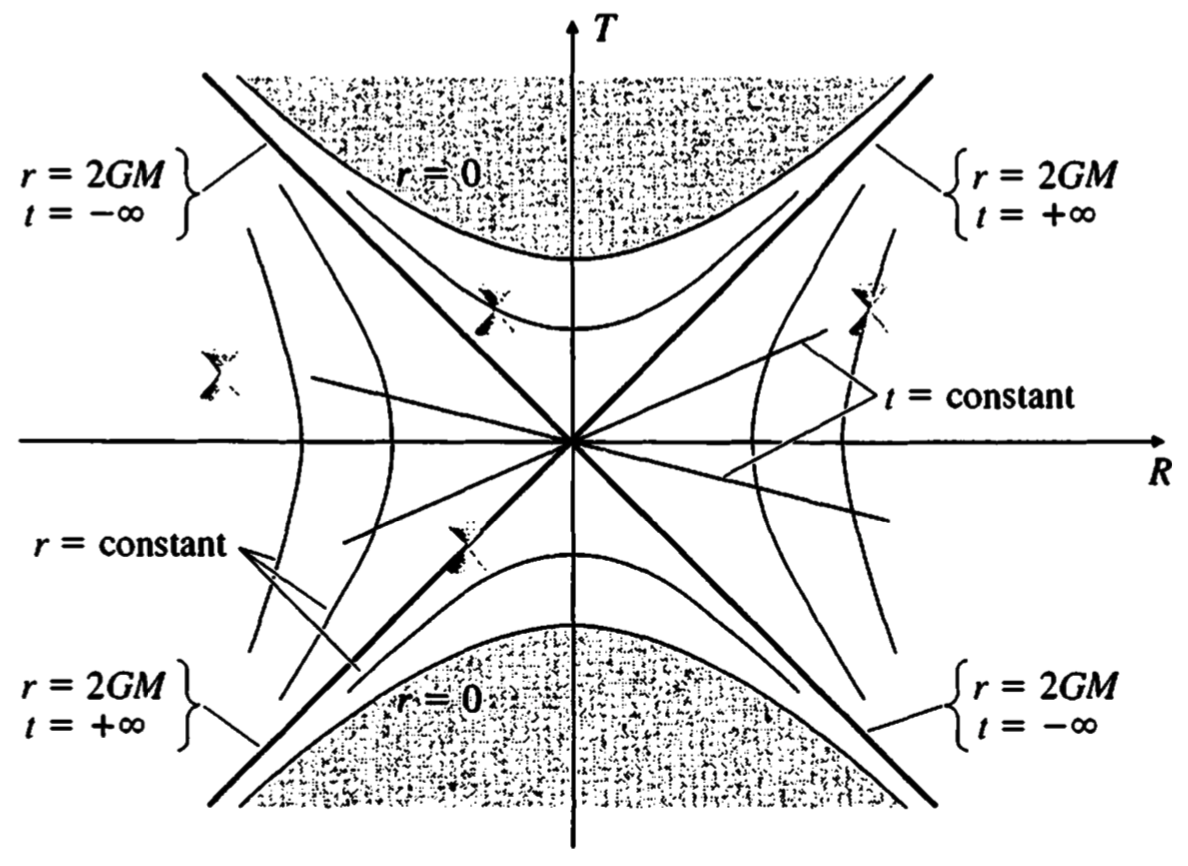
\includegraphics[scale=0.2]{carroll_fig_5_12.png} 
%\end{center}
\caption{Kruskal diagram of Schwarzschild black hole [1].}
\end{figure}

The Kruskal diagram separates spacetime into 4 regions, shown in Figure \ref{fig:kruskalregions}. Region I is our universe. Region II is inside the black hole, with its singularity along the border of the shaded region. Region III is a white hole, a time-reversed copy of a black hole. Region IV is a mirror-image of our universe, which can only be reached from Region II by travelling faster than the speed of light. Theoretically, regions II and IV are connected by a wormhole.
light rays make $45\degree$ lines.
\begin{figure}[h]\label{fig:kruskalregions}
\centering
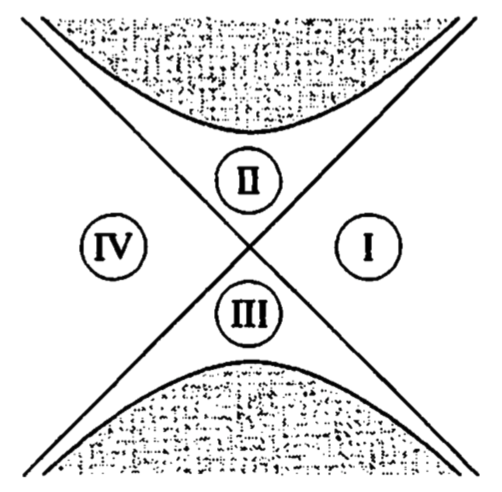
\includegraphics[scale=0.25]{carroll_fig_5_13.png}
\caption{Regions of Kruskal diagram. [1]} 
\end{figure}

\newpage
\section{References}
[1] S. Carroll, Spacetime and Geometry (Addison-Wesley,
2003).

\end{document}
